%
% File emnlp2019.tex
%
%% Based on the style files for ACL 2019, which were
%% Based on the style files for EMNLP 2018, which were
%% Based on the style files for ACL 2018, which were
%% Based on the style files for ACL-2015, with some improvements
%%  taken from the NAACL-2016 style
%% Based on the style files for ACL-2014, which were, in turn,
%% based on ACL-2013, ACL-2012, ACL-2011, ACL-2010, ACL-IJCNLP-2009,
%% EACL-2009, IJCNLP-2008...
%% Based on the style files for EACL 2006 by 
%%e.agirre@ehu.es or Sergi.Balari@uab.es
%% and that of ACL 08 by Joakim Nivre and Noah Smith

\documentclass[11pt,a4paper]{article}
\usepackage[hyperref]{emnlp-ijcnlp-2019}
\usepackage{times}
\usepackage{latexsym}
\usepackage{graphicx}  %%% for including graphics
\usepackage{booktabs}
\usepackage{xspace}

\usepackage{url}

%\aclfinalcopy % Uncomment this line for the final submission

%\setlength\titlebox{5cm}
% You can expand the titlebox if you need extra space
% to show all the authors. Please do not make the titlebox
% smaller than 5cm (the original size); we will check this
% in the camera-ready version and ask you to change it back.

\newcommand\BibTeX{B{\sc ib}\TeX}
\newcommand\confname{EMNLP-IJCNLP 2019}
\newcommand\conforg{SIGDAT}
\newcommand{\refexp}[1]{\textsl{#1}}
\newcommand{\word}[1]{\textsl{#1}}
\newcommand{\cat}[1]{\textsc{#1}}
\newcommand{\vgenome}{VisualGenome\xspace}
\newcommand{\ra}{$\rightarrow$}

\newcommand{\sz}[1]{\textcolor{blue}{\emph{//sz: #1//}}}
\newcommand{\gbt}[1]{\textcolor{orange}{\emph{//g: #1//}}}
\newcommand{\cs}[1]{\textcolor{green}{\emph{//cs: #1//}}}

\title{Do Objects in Real-World Images Have a Canonical Name?} 

\author{First Author \\
  Affiliation / Address line 1 \\
  Affiliation / Address line 2 \\
  Affiliation / Address line 3 \\
  {\tt email@domain} \\\And
  Second Author \\
  Affiliation / Address line 1 \\
  Affiliation / Address line 2 \\
  Affiliation / Address line 3 \\
  {\tt email@domain} \\}

\date{}

\begin{document}
\maketitle

\begin{abstract}
In research on language \& vision, it is well known that different speakers interpret and describe the same visual scene in many different ways.
Individual visual objects, however, are usually simply annotated with a single canonical name, assuming that linguistic variants of the canonical name that would occur in natural naming situations (e.g. when referring to the object) can be retrieved from a taxonomy like WordNet.
We put these assumptions to an empirical test and elicit (from 36 subjects) a dataset of non-canonicalized object names on top of 25k objects of the VisualGenome dataset. 
Our results reveal a manageable amount of variation in names given to individual objects (approx. 3 different types on average), and wide variation in names for objects of the same category (around 30 different names for categories like e.g.\ dog).
%\cs{Is with category ANIMAL meant, or more dog --> many images of dog, high variation?}
%\cs{Should it made explicit that most instances have more than one name?}
%\cs{What does "decent" mean?}
We observe that most of the alternatives for the canonical VisualGenome name cannot be retrieved via hierarchical relations encoded in WordNet. 
Instead, a major portion of the variation is accounted for by more complex relations like cross-classification of objects, metonymy or variation due to visual uncertainty.  
We investigate whether a state-of-the-art model of object labeling implicitly encodes similar variation in object naming and discuss implications for research in language \& vision.
\end{abstract}

\section{Introduction}
\begin{figure}[tbp]
\begin{tabular}{p{2.5cm}p{2.5cm}}
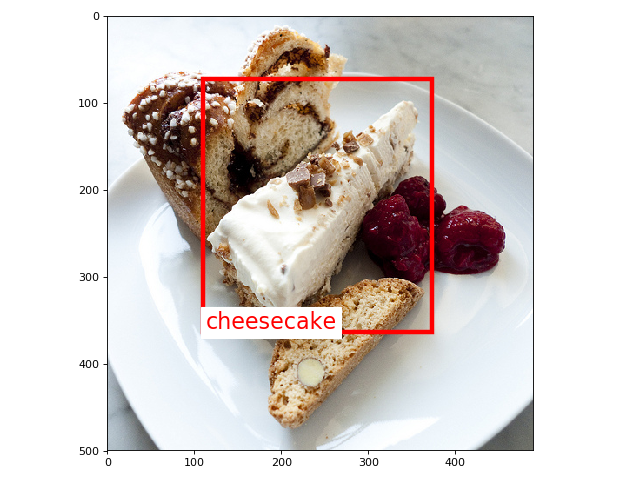
\includegraphics[height=3cm]{figures/cheesecake.png} &
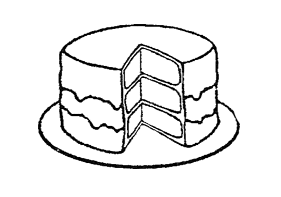
\includegraphics[height=3cm]{figures/snodgrass_vanderwart_cake_042.png}
\end{tabular}
\caption{Object name from VisualGenome. Names like \refexp{cake}, \refexp{dessert}, \refexp{sweet}, or \refexp{food} would be valid, too.}
\label{fig:cake}
\vspace{-0.5cm}
\end{figure}

Determining object names, such as \emph{cheesecake} for the marked object in Figure~\ref{fig:cake}, is a core aspect of virtually every language \& vision task, ranging from e.g.\ referring expression generation to visual dialogue \cite{fangetal:2015,devlin:imcaqui,Bernardietal:automatic,das2017visual,vries2017guesswhat}.
%While many of these tasks are well-known to 
%\gbt{I've left only one image in the figure to highlight that we study variation for the same instance.}
However, so far research in NLP has had surprisingly little to say about object naming.
Neighboring areas
%, specifically Computer Vision and Cognitive Science, 
have addressed related tasks, with simplifications that NLP is equipped to address:
In Computer Vision, naming is usually equated with object categorization, and addressed as a classification problem in which a single label is provided for each object~\cite{googlenet}.
%In a typical evaluation, alternative names for the object in Figure \ref{fig:cake} such as \refexp{cake}, \refexp{dessert}, \refexp{sweet}, or \refexp{food} would be counted as incorrect.
In Cognitive Science, object naming has received more attention, but it has been studied with stylized drawings instead of realistic images.
%, such that it is unclear how findings generalize to tasks in language \& vision.

We take a first step at studying naming of object in real-world images and contribute a new dataset, ManyNames, that contains 36 crowd-sourced names for 25K instances from VisualGenome~\cite{krishna2016visualgenome}.
Thus, our images show objects in complex visual contexts
%, surrounded by other objects, 
unlike the ``clean'' ImageNet data~\cite{imagenet_cvpr09} that has been previously used to train object or name classifiers \cite{Ordonez:2016}.

We find both consistency and variation in naming: In instances, the relative frequency of the most common name is 75\% on average, which is remarkable for a task where subjects are allowed to produce whatever name they like.
However, 
%there are still around 3 names being produced for each instance on average.
%Moreover, 
we find a high level of variation within what would be considered a class in visual object recognition, with around 30 names per class.
%standard Computer Vision approaches (objects assigned the same synset in VisualGenome)
Interestingly, most of this variation comes from alternative names that do not stand in a taxonomic relation, but range from 
%We also find a very high standard deviation in the agreement measures, which suggests that visual features (how prototypical the instance is of a given category, how clearly delimited the object is) are crucial factors determining variation.
%Our data also show that object identification via bounding boxes is not a trivial matter even for humans, with name variants ranging from clearly different objects in 
cross-classifification  (\textit{cheesecake}-\textit{dessert}) to cases
% where it is visually impossible to distinguish between the two (\textit{bed}-\textit{bedsheet} when the bed is only partially shown) to cases 
of near-metonymy (\textit{floor}-\textit{carpet}) and issues in object idenitification due to bounding boxes (\textit{man}-\textit{helmet}).
%Given these findings, we ask whether current models implicitly capture object naming variation of the sort provided by humans.
When testing a model of object classification trained on VisualGenome on ManyNames, we observe  better performance performs than on VisualGenome: It has 77\% accuracy when taking the most frequent ManyNames name as gold standard, vs.\ only 69\% on the VisualGenome name.
This suggests that object names annotated by many speakers provide a more robust ground for testing computational models, while also offering rich data for studying linguistic variation in naming.
%\gbt{Not sure what to say about variation proper}

% \item most of the variation in our dataset comes from alternative names that do not stand in a taxonomic relation, suggesting that the previous work in Cognitive Science is missing much of the empirical ground.
% %while previous work has mostly focused on variation in the level of generality within a taxonomy (\emph{penguin} vs. \emph{bird}), 

% our datasets contains a lot of variability for names coming from different parts of the taxonomy (\emph{dessert} vs. \emph{cake}, \emph{bottle} vs. \emph{wine})
% \end{itemize}

% Moreover, we analyze whether current models implicitly encode the variation in naming, by doing XXX. We find YYY.


% Our paper puts together two strands of research that have mostly been pursued independently to date.
% On the one hand, state-of-the-art computer vision systems are able to accurately classify images into thousands of different categories (e.g.\  \newcite{googlenet}), where the task is often to predict the class for a given object. 
%name for a given object. \gbt{Is this true? Imagenet task asks for synsets, which can be taken to be categories\dots To refine}
% However, they mostly adopt very simple assumptions with respect to the underlying lexicon, which is implemented by using single "ground truth" labels: 
%as a simple, flat labeling scheme:
 % A standard object recognition system would be trained to classify the left object in Figure~\ref{fig:cake} as \emph{cheesecake}, the right one as \emph{dessert}, and using \emph{dessert} for the left picture would be considered incorrect. 
% On the other hand, research on object naming in Cognitive Science has shown that people choose different names depending on the circumstances, with factors such as context or the prototypicality of the object with respect to the category playing a role~\cite{add-refs}. 
% \gbt{This research also argues that there is high agreement in how people name objects; to do: make coherent.}
% However, this research typically uses stylized drawings are used, and is focused on taxonomic relations (\textit{sparrow}-\textit{bird}).
% \sz{It is thus unclear how findings from these stylized settings generalize to tasks in language \& vision like referring expression generation, where naming is a core aspect. Therefore, in contrast to traditional naming norm studies in Cognitive Science we study object naming in realistic scenes where objects are situated in a natural context! (This comes with additional challenges, like potential object occlusion, background/foreground confusion etc.)}

% Seminal work on prototypes suggests that the prototypicality of the object will determine the level of generality of the object name, i.e.\  a robin can be named \emph{bird}, but a penguin is better referred to as ``\emph{penguin}'' \cite{Rosch1978}.

% Two main findings in the literature:

% \begin{itemize}
% \item very high agreement, most people use the same name for the same object
% \item prototypicality is a factor, context too, but research has only looked at generality/specificity of the name
% \end{itemize}

%The real-world objects that we interact with in our every-day life can be categorized into many thousands and maybe millions of categories. And even a single object can be member of many categories, i.e.\ at different taxonomical levels or in different parts of a taxonomy. For instance, both objects in Figure \ref{fig:cake} are at once instances of \cat{cake}, \cat{cheesecake}, \cat{dessert}, \cat{sweet}, \cat{pastry}, \cat{food} etc. Hence, when speakers name objects, e.g.\ when referring, they have to select a lexical item from a complex network of concepts and competing lexical alternatives.

%To date, research in NLP has surprisingly little to say about object naming, despite the fact that
% there has been a recent explosion of interest in various, and even complex, language \& vision tasks ranging from image captioning \cite{fangetal:2015,devlin:imcaqui,Bernardietal:automatic} to e.g.\ visual dialogue \cite{das2017visual,vries2017guesswhat}. 
%In contrast, closely related areas, such as computer vision and cognitive science, have investigated very related tasks in quite some depth: object recognition systems developed in the area of computer vision  are now able to classify images into thousands of different categories (e.g.\  \newcite{googlenet}).
%Furthermore, work on concepts, following the seminal work by Rosch, suggests that objects are typically conceptualized at a preferred level of specificity called the \textbf{entry-level}. Psycho-linguistic studies have been able to support this theory based on collections of so-called object naming norms. 
%
%This paper aims at addressing the genuinely linguistic questions revolving around the phenomenon of object naming by (i) presenting a collection of high-quality, large-scale naming data,  and (ii) analysis methods for this data and (iii) a first baseline model that accounts for the semantic flexibility of names for objects in real-world images. From computer vision, we borrow the idea of modeling realistic visual objects in realistic scenes (real-world images), but go beyond the simplistic assumption that object names correspond to unambiguous labels in a flat classification scheme (with no conceptual relations between the labels). From psycholinguistics, we borrow the idea of eliciting natural, representative naming data from many subjects, but go beyond using artificial, highly stylized objects.

%%% Local Variables:
%%% mode: latex
%%% TeX-master: "main"
%%% End:


%\section{Related Work}
%\label{sec:relwork}
%\paragraph{Cognition: Concepts and categorization}

 Seminal work on concepts by Rosch and colleagues suggests that object names typically exhibit a preferred level of specificity, which \citet{jolicoeur1984pictures} called the \textbf{entry-level}. This typically corresponds to an intermediate level of specificity, i.e., \textbf{basic level} (e.g, \refexp{bird}, \refexp{car}) \cite{rosch1976basic}, as opposed to more generic (i.e., \textbf{super-level}; e.g., \refexp{animal}, \refexp{vehicle}) or specific categories (i.e., \textbf{sub-level}; e.g., \refexp{sparrow}, \refexp{convertible}). However, less prototypical members of basic-level categories tend to be instead identified with sub-level categories (e.g., a \cat{penguin} is typically called a \refexp{penguin} and not a \refexp{bird}) \cite{jolicoeur1984pictures}. 
%This out-of-context preference towards a certain taxonomic level is often referred to as \textbf{lexical availability}. 
While the traditional notion of entry-level categories suggests that objects tend to be named by a \refexp{single} preferred concept, research on pragmatics has found that speakers are flexible in  
%with respect to the chose level of specificity. 
their choice of the level of specificity. 
Scenarios where multiple objects (of the same category) are present induce a pressure for generating names which uniquely identify the target \cite{olson1970language}, such that sub-level names can be systematically elicited in these cases %\cite{rohde2012communicating} \cite{graf2016animal}. 
\cite{rohde2012communicating,graf2016animal}.

\paragraph{Vision: Object Recognition}

State-of-the-art computer vision systems are able to classify images into thousands of different categories (e.g.\  \newcite{googlenet}). These object recognition systems are now widely used in vision \& language research.
Nevertheless, the way the treat object recognition is conceptually very simple (if not to say, naive):  standard object classification schemes are inherently ``flat'', and treat object labels as mutually exclusive \cite{deng2014large}, ignoring all kinds of linguistic relations between these labels and ignoring the fact that an object can easily be an instance of several categories.\cs{I would make this statement stronger and argue that \textbf{object recognition is merely a labeling of objects  with human interpretable symbols}, and that a system would probably fail if it had to decide whether an object labeled as, e.g.\ \refexp{fig} may also be labeled as \refexp{food}.} \gbt{ok}


\paragraph{Vision \& language: Naming and Referring}

\newcite{Ordonez:2016} have studied the problem of deriving appropriate object names, or so-called entry-level
 categories, from the output of an object recognizer. Their approach focusses on linking abstract object categories in ImageNet to actual words via translation procedures that e.g. involve corpus frequencies. 
 \newcite{zarriess-schlangen:2017} learn a model of object naming on a corpus of referring expressions paired with objects in real-world images, but focus on combining visual and distributional information and on zero-shot learning.
Object naming is also an important task for referring expression generation, though most research in this area has focussed on content and attribute selection \cite{Kazemzadeh2014,gkatzia:2015,zarrieschlang:easy-pre,Maoetal:cocorefexp}. \gbt{Should we put this as motivation also in the intro?}

% \paragraph{Existing resources and their shortcomings}
% Moreover, existing resources in L\&V hardly provide any consistent taxonomic information on objects and their categories, e.g. object labels are typically quite general as in Flickr30k \cite[e.g.,~\cat{people, animals, bodyparts, clothing}]{plummer2015flickr30kentities} or taxonomically heterogeneous as in MS COCO \cite[e.g.,~\cat{people, baseball glove, bird}]{mscoco}.


%%% Local Variables:
%%% mode: latex
%%% TeX-master: "main"
%%% End:


\section{Data collection}
%\label{sec:data}
%% Number of images/objects:        25,596\\
% Number of object names:  450\\
% Number of collection nodes (synsets):    52 \\

\begin{table*}[htp]
	\small
	\centering
	\begin{tabular}{lp{14cm}}
			\toprule
			Domain & \multicolumn{1}{c}{Collection synsets}\\
			\midrule			
			animals\_plants & ungulate$_1$ (2037), horse$_1$ (833), feline$_1$ (763), dog$_1$ (688)
			bird$_1$ (389), flower$_1$ (44), rodent$_1$ (27), insect$_1$ (12), fish$_1$ (11)\\
			buildings      &  house$_1$ (364), bridge$_1$ (297), shelter$_1$ (169), restaurant$_1$ (58),
                                         outbuilding$_1$ (31), hotel$_1$ (19), housing$_1$ (17), place\_of\_worship$_1$ (12)     \\
			clothing       &  shirt$_1$ (968), overgarment$_1$ (786), dress$_1$ (199), headdress$_1$ (135),
                                         neckwear$_1$ (65), robe$_1$ (27), glove$_2$ (7), footwear$_1$ (5)    \\
			food           &  dish$_2$ (812), baked\_goods$_1$ (770), foodstuff$_2$ (280), vegetable$_1$ (48),
                                         edible\_fruit$_1$ (42), beverage$_1$ (23)   \\
			home           &  furnishing$_2$ (5,355), vessel$_3$ (525), kitchen\_utensil$_1$ (132), crockery$_1$ (92),
			cutlery$_2$ (82), tool$_1$ (72), lamp$_1$ (34)    \\
			people         & woman$_1$ (1768), man$_1$ (1167), male\_child$_1$ (853), athlete$_1$ (396),
			 child$_1$ (333), creator$_2$ (11), professional$_1$ (5)    \\
			vehicles       &  aircraft$_1$ (1208), train$_1$ (957), car$_1$ (727), motorcycle$_1$ (564),
                                         truck$_1$ (559), boat$_1$ (499), ship$_1$ (38)    \\
			\bottomrule
		\end{tabular}
		\caption{Overview of the ManyNames dataset: Synset nodes for each domain (subscript indicates synset number; number of instances in parentheses).
                  \label{tab:overview_dataset2}}
	\end{table*}

\begin{table*}[htp]
	\small
	\centering
	\begin{tabular}{@{~}l@{~}l@{~}l@{~}l@{~}l@{~}l@{~}l}
		\toprule
		vehicles &            food & animals\_plants &           home &        buildings &             people &      clothing \\
		\midrule
		train (954) &  pizza (518) &  giraffe (915) &  bed (888) &  house (340) &  boy (853) &  shirt (904) \\
		car (642) &  cake (261) &  horse (822) &  bench (714) &  bridge (274) &  man (806) &  jacket (451) \\
		plane (485) &  bread (186) &  cat (754) &  table (687) &  dugout (91) &  woman (766) &  coat (267) \\
		airplane (479) &  sandwich (153) &  dog (654) &  desk (672) &  tent (53) &  girl (650) &  dress (190) \\
		motorcycle (466) &  bun (143) &  zebra (461) &  counter (516) &  restaurant (33) &  lady (342) &  hat (77) \\
		% truck (465) &  cheese (110) &  cow (324) &  couch (366) &  overpass (23) &  guy (330) &  t-shirt (62) \\
		% boat (450) &  donut (78) &  bird (295) &  chair (365) &  grill (22) &  child (230) &  tie (51) \\
		% jet (106) &  salad (70) &  sheep (216) &  carpet (307) &  garage (18) &  batter (110) &  blazer (43) \\
		% aircraft (85) &  sauce (68) &  bull (48) &  bowl (219) &  hotel (16) &  kid (85) &  hood (26) \\
		% van (76) &  apple (33) &  flower (40) &  curtain (182) &  castle (14) &  skateboarder (80) &  cap (20) \\
		\bottomrule
	\end{tabular}
	\caption{Overview of the ManyNames dataset: Top 5 VG names for each domain (number of instances in parentheses).\label{tab:overview_dataset1}}
\end{table*}

\begin{figure*}[htp]
  \centering
  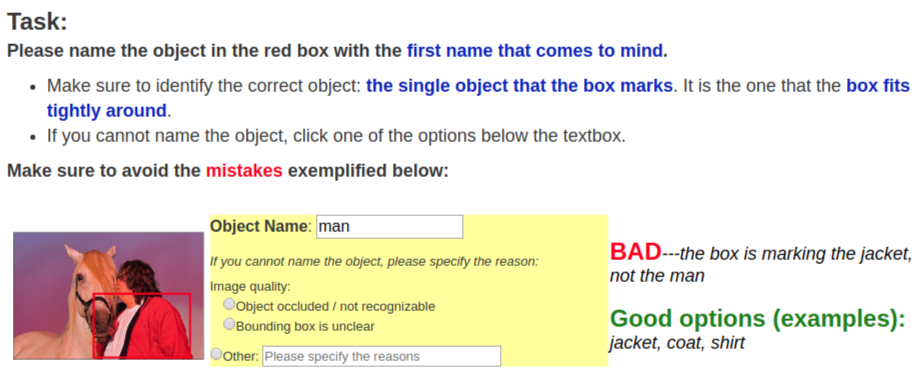
\includegraphics[width=1.5\columnwidth]{figures/round0_cropped.png}
  \caption{Instructions for AMT annotators for the first round (whole instructions showed more examples, see Figure~\ref{fig:instructions2}).}
  \label{fig:instructions1}
\end{figure*}

We take data from \vgenome~(VG, \newcite{krishna2016visualgenome}), which
contains a dense region-based labeling of $108$K~images with, inter alia, object names, attributes and relationships,
all linked to WordNet synsets \cite{fellbaum1998wordnet}.
\vg suits our purpose of collecting names for naturalistic instances of common objects, as it has images of varying complexity, with close-ups as well as images with many objects.
As common in Computer Vision, objects are localized as bounding boxes, as in Figure~\ref{fig:cake}.% 
\footnote{We use image and object interchangeably in the following, since we only selected one target object per image (i.e., each object and image in VG is chosen at most once).}

\subsection{Sampling of Instances}
\label{ssec:sampling}

%Criteria: From CV: select images depicting objects with relatively frequent names; From CogSci: select objects which have been frequently studied in cognitive science/psychological norming studies; we chose McRae et al. as basis.
We selected images from seven domains: \domain{animals\_plants}, \domain{buildings}, \domain{clothing}, \domain{food}, \domain{home}, \domain{people}, \domain{vehicles}. 
They are all based on McRae et al.'s  \cite{mcrae2005semantic} feature norms, a dataset widely used in Psycholinguistics that comprises common objects of different categories, except for \domain{people}, which we added because it is a very frequent category in \vg and a very prominent category for humans.
% We start from the concepts of McRae et al.'s feature norms (REF), which are common objects of different categories (e.g.,~\domain{animals}, \domain{furniture}) and, as such, have a high overlap with standard datasets of object norming studies (REFS).
% We added the \domain{person} category because it is very frequent category in \vgenome.

Within each domain, we aimed at collecting instances at different taxonomic levels to cover a wide range of phenomena, but this is not straightforward because ontological taxonomies do not align well with the lexicon (for instance, \textit{dog} and \textit{cow} are both mammals, but \textit{dog} has many more common subcategories), and most domains are not organized in a clear taxonomy in the first place (e.g.\ \domain{home}).
Instead, we defined a set of synsets ($52$\ in total; listed in Table~\ref{tab:overview_dataset2}) that we used to collect object instances from \vg, as follows. 

First, to create our synset set, we chose those \vg synsets that match or subsume the object classes in the McRae norms, and have a high number of \vg object instances of different names.\cs{prev. sentence this is still a bit fluffy}
For example, \vg instances subsumed by McRae's \textsl{dog} were named \textsl{beagle, greyhound, puppy, bulldog}, etc., while McRae's \textsl{duck}, \textsl{goose}, or \textsl{gull} did not have name variants in \vg, so we kept \textsl{dog} and \textsl{bird} (which subsumes \textsl{duck}, \textsl{goose}, or \textsl{gull}) as collection synsets.
%\gbt{Just to clarify: we also collected objects named \textsl{duck}, \textsl{goose}, or \textsl{gull}, right? Not only \textsl{bird}?}

We then retrieved all VG images depicting an object whose name matches or is subsumed by words in one of these synsets; we refer to these words as \textit{seeds} ($450$\ in total).
\gbt{from the dataframe in the github it's 449. Also, there are some mistakes in the list of seeds ('dugout.', 'man's') -- to check after the deadline.}
We did not consider objects with names in plural form, with parts-of-speech other than nouns\footnote{We obtained tags with CoreNLP \cite{manning2014stanford}.}, or that were multi-word expressions (e.g.,~\textsl{pink bird}). 
We further only considered objects whose bounding box covered~\mbox{$20-90\%$} of the image area.
% We based the definition of our set of nodes on the WN (REF) synsets of the McRae concepts (e.g.,~dog, duck, goose, gull), the nominal WordNet hierarchy, and the frequency distribution of the VG object names' synsets.\footnote{TODO: need to be clear from the general description of VG that the frequ. of instances labeled with the synset of the object name is meant.} 
% First, we selected a set of collection node candidates---synsets which match (e.g.,~\textsl{dog, duck, goose, gull}) or subsume (e.g.,~\textsl{mammal, bird}) the McRae synsets\footnote{Specific synset IDs, e.g.,~dog.n.01, are omitted for readability.}. 
% From these candidates we kept those as collection nodes which had a high frequency of VG object instances of different names. For example, VG instances  subsumed by McRae's \textsl{dog} were named \textsl{beagle, greyhound, puppy, bulldog}, etc., while McRae's \textsl{duck, goose}, or \textsl{gull} did not have name variants in VG, so we kept \textsl{dog} and \textsl{bird} as collection nodes.
%\paragraph{Collection of instance candidates}
% Goal of above procedure was the collection of instances of selected object classes---our nodes--- whose VG names correspond to or subsume (are hypernyms of) a McRae concept, and whose object names differ, that is, of which we can expect that people possess different names for them (e.g.,~\textsl{duck, goose, gull} for \textsl{bird}).
% \paragraph{Sampling of instances}
Because of the Zipfian distribution of names, and to balance the collection, we sampled instances depending on the size of the seeds: up to $500$\ instances for seeds with up to $800$\ objects, and up to $1000$\ instances for larger seeds. This yielded a dataset of\ $31,093$~instances, which was further pruned during annotation, as explained next.
Table~\ref{tab:overview_dataset1} shows the top 5 \vg names in each of the domains.

\subsection{Elicitation Procedure}
\label{ssec:elicitation}

To elicit object names, we set up a crowdsourcing task on Amazon Mechanical Turk (AMT).
In initial pilot studies, we found object identification via bounding boxes to be problematic.
In some cases, the bounding box was not clear; in others, AMT workers named objects that were more salient than the one signaled by the box (for instance, for a box around a jacket, the man wearing it).
We took special care of minimizing this issue in two ways: Specifying the instructions such that workers pay close attention to what object is being indicated in the box, and pruning images with unclear boxes or occluded objects via an initial collection round in which we allowed workers to mark such cases.
Figure~\ref{fig:instructions1} shows the task instructions for this first round, in which 9 workers annotated each image.

%We eliminated around $5.5$K\ images based on pruning, obtaining the final dataset with $25,596$\ images.
After the first round, and based on the opt-out annotation, we kept images that met all the following conditions (thresholds were estimated via manual inspection): (i) they were not marked as occluded by any subject; (ii) ``Bounding box is unclear'' was marked at most twice; (iii) at most 17\% of elicited names were in plural form (to remove cases where the bounding box contains several objects); (iv) the most frequent elicited name is of the same domain as the \vg name.
This yielded $25,596$ images (we discarded $5,497$).
We then did 3 more collection rounds, obtaining a total of 36 images per object.
Figure~\ref{fig:instructions2} shows the instructions for these rounds; they were accompanied by a FAQ solving common issues. 
We shuffled the set of images per task between rounds, and workers could only participate in one round, to avoid workers annotating an instance more than once.
Overall $841$\ workers took part in the data elicitation, with a median of  $261$\ instances \mbox{($\textrm{range}=[9,17K]$)} per worker.

\begin{figure*}[htp]
  \centering
  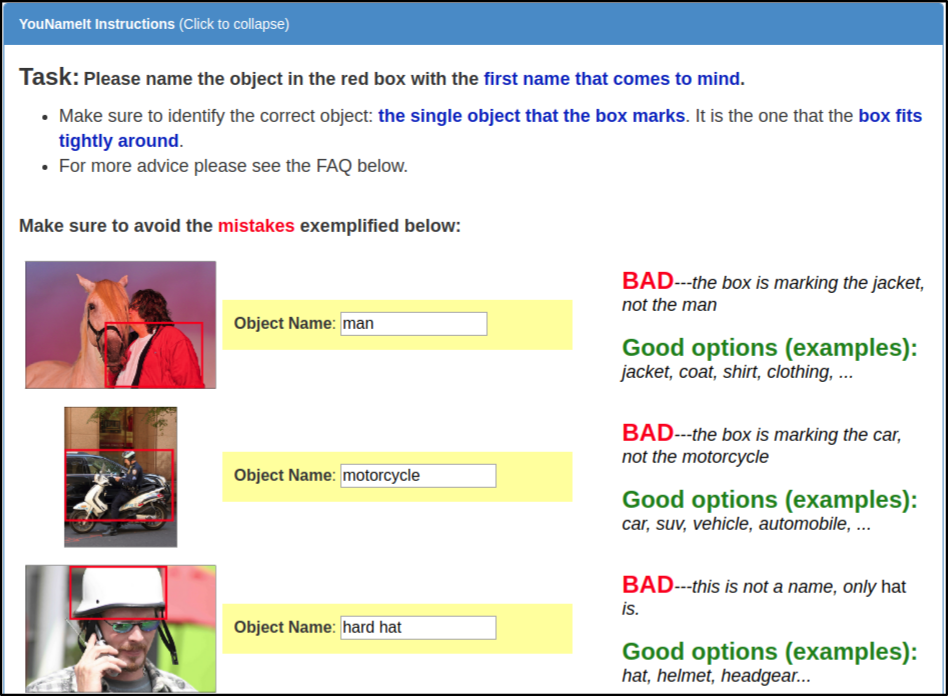
\includegraphics[width=1.5\columnwidth]{figures/round1+_p1.png}
  \caption{Instructions for AMT annotators for rounds~$2$ to~$4$.}% They were accompanied by the FAQ in Figure~\ref{fig:faq}}
  \label{fig:instructions2}
\end{figure*}

% \begin{figure*}[htp]
%   \centering
%   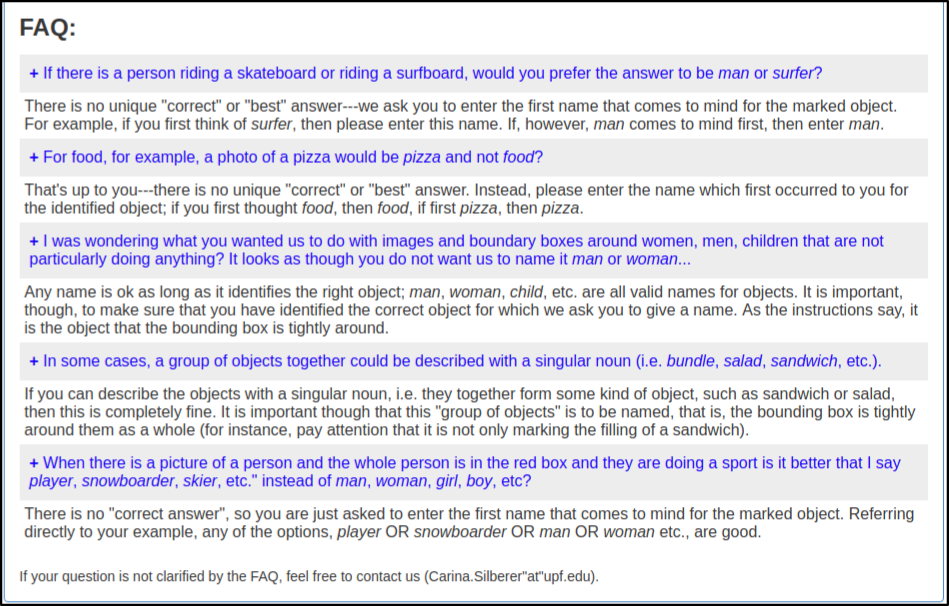
\includegraphics[width=1.5\columnwidth]{figures/round1+_p2.png}
%   \caption{FAQ accompanying the instructions for AMT annotators for rounds~$2$ to~$4$.}
%   \label{fig:faq}
% \end{figure*}

%\cs{Maybe say something about the rejections, if space permits it.}

%%% Local Variables:
%%% mode: latex
%%% TeX-master: "lrec2020naming"
%%% End:




\section{Analysis: Agreement}
\label{sec:analysis}
%\gbt{Points to discuss in the paper, as discussed with Carina May 16:}
%
%\begin{itemize}
%\item Super high variance in the agreement. Higher agreement for instances, lower for classes. Suggests systematicities at the instance level that do not depend on the class. Hypothesis, supported by qualitative analysis (Figure 3): relevance of visual perceptual factors. E.g.: saliency, background/foreground (desk-keyboard; bridge-train); ``angle'' from which the object is shown (see girl-t-shirt example); \dots In addition, we also find aspects discussed by Psycholing, but at the level of the instance: Typicality (see truck-bus example, bridge-dock, bench-seat). 
%\item Forget about WordNet.
%\item Implications for lang\&vision: 1) synset classification won't do (if the goal is to predict/label an object); 2) name classification won't do either; 3) ``mistakes'' done by models are also done by humans -- role of referential uncertainty.
%\end{itemize}


In this section, we investigate to what extent names annotated in VisualGenome and elicited in ManyNames can be considered canonical, i.e. to what extent speakers agree in their naming choices.
Whereas traditional picture naming studies typically use a prototypical image per category (see Figure~\ref{fig:picture_naming}) and, hence, are mostly interested in the agreement on concept or category-level, we carry out an analysis on two different levels: First, we will look at instances and see to what extent names overlap for the same object. 
Second, we will use the existing annotation of names in VisualGenome to analyze agreement on the level of classes.
\begin{figure}[t]
	\centering
	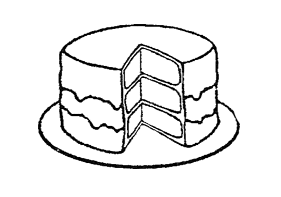
\includegraphics[scale=.5]{figures/snodgrass_vanderwart_cake_042.png}
	\caption{Example of a picture of \textsl{cake} used in traditional picture naming studies (REF to Vanderwart \& Snodgrass) \label{fig:picture_naming}}
\end{figure}

\subsection{Names, instances, classes}

First of all, to see whether objects in ManyNames bear a canonical name, we simply count how many different names (i.e.\ types) are given to instances, and to all instances that have the same synset annotated in VisualGenome. 
As the data is collected via crowdsourcing and a certain amount of noise is to be expected, we apply different frequency thresholds on the response sets for instances and synsets.
Figure \ref{fig:ntypes} shows the cumulative histograms for type counts, obtained with different thresholds (from 1 to 6).
Without any frequency thresholding, the proportion of instances and classes that have a single name annotated is small, i.e.\ below 10\% in both cases. When raising the threshold up to a minimum of 4 occurences in the response set  for instances (meaning more than 10\% of the 36 annotations), the proportion of objects that really only have a single name annotated is considerably higher, but still below 50\%.
Thus, as expected in a free annotation scenario, the MN data contains a certain number of low-frequency responses.
The fact that even after applying a relatively strict frequency filter most objects have more than one name annotated indicates that there is a non-negligible  level of variation when different speakers name the same object.

The amount of variation increases substantially when looking at the number of names we find for different synsets in Visual Genome, as is indicated by the histogram for type counts of synsets in Figure \ref{fig:ntypes}.
Here, we observe that the rise of the curve is much less steep than for instances and, generally, there are many synsets with more than 10 or even 20 different name types, even after applying the frequency threshols.

\begin{figure*}
\begin{minipage}[b]{0.4\linewidth}
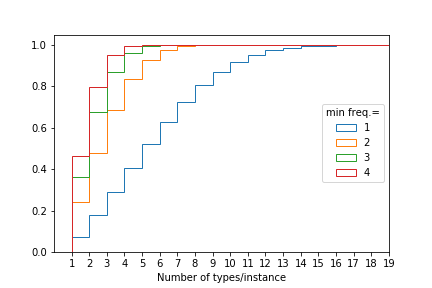
\includegraphics[scale=.4]{Figures/types_instances.png}
\end{minipage}
\begin{minipage}[b]{0.6\linewidth}
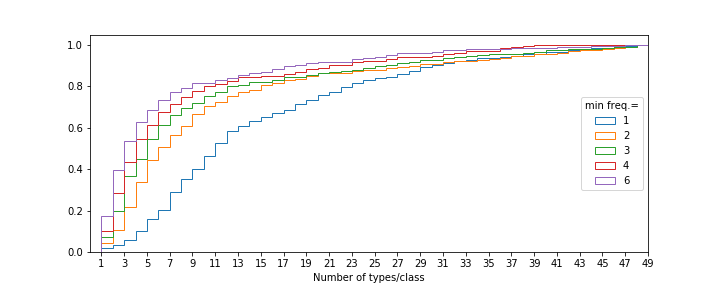
\includegraphics[scale=.4]{Figures/types_classes.png}
\end{minipage}
 \caption{\label{fig:ntypes} Cumulative histograms for number of types found for instances and classes, based on different frequency tresholds (applied on the level of instances and classes respectively)}
\end{figure*}


\subsection{Agreement}

We compute the following agreement measures:

\begin{itemize}
\item \textbf{\% top}: the average relative frequency of the most frequent response (shown in percent)
\item \textbf{$H$}: the $H$ agreement measure used previously in the psycholinguistic literature
\cs{How is this defined?}
\begin{equation}
H = \sum_{i=1}^k p_i\ log_2(1/p_i)
\end{equation}

\item \textbf{N}: the average number of types in the response set of ManyNames
%\item \textbf{N$_{>1}$}: the average number of types, excluding types that have been annotated only once
\cs{alternatively we could show a plot going from 1 to, let's say, $>10$}
\item \textbf{top=VG}: the proportion of items where the top response in ManyNames corresponds to the VisualGenome name
\item \textbf{\% VG}: the average relative frequency of the VisualGenome name in the response set

\end{itemize}

For measuring \textbf{instance-level agreement}, we consider all names annotated for an object as a response set and then average over these response sets. Furthermore, we compute \textbf{class-level agreement} by merging the response sets for all objects that have the same synset (given for the original VisualGenome name) and compute the measures over these aggregated response sets.
\gbt{@Sina, what are the synsets that you got here? Are they collection nodes, or the synset of the VG name as annotated in VG?}


Table \ref{tab:agree} shows the analysis of the instance-level and category-level agreement.
On the instance-level, our annotators achieve a fair amount of overlap in their object naming choices. 
Thus, for roughly 70\% of our objects (\textbf{std=?}), the most frequent response in ManyNames corresponds to the original VisualGenome name and, similarly, the average frequency of the top response is also 70\%. 
%Generally, this seems to suggest that indeed many objects in our data set have a canonical name. 
\sz{For NLP people, this looks like a good agreement (given that people were free to type what they wanted). For vision people who might think of it as an object labeling task, this would be pretty low/bad agreement.}
At the same time, the average number of name types per object (5.7, or 2.9 when excluding low-frequency types in each response set) suggests that there is a stable amount of naming variants that is elicited for instances. 
Furthermore, the agreement varies quite considerably among domains \cs{refer to std}:  in the animal domain, which is often discussed in the object naming literature, annotators achieve a very stable and robust agreement of over 90\% and an $H$ agreement which comes close to 0 (where 0 is perfect agreement). 
The people domain, on the other hand, is subject to much more variation and agreement is dramatically lower here, and comes close to 50\% for \% top.



%\gbt{Super-interesting results.}
Finally, the category-level agreement figures tell yet another story: when aggregating the responses for all objects with the same VisualGenome synset, we obtain on average 30 types (with $N_{>1})$, i.e. variants of the original VG class. 
Surprisingly, here, only 32.7\% of the aggregated response sets still have the VG name as the most frequent response, which means that for 70\% of the VG names, annotators in ManyNames, on average, prefer a different name.  
Likewise, the relative frequency of the top response drops considerably and $H$ increases from 1.3 for instance-level agreement to 2.4 on object-level agreement.  
%\cs{Can we say more about what's going on in the people and vehicles domain, category-level, top=VG? E.g., put corresponding examples in Tab.\ref{tab:qual}}
%

\subsection{Variation and WordNet}

Previous work on large-scale collections of labels or names of objects has (explicitly or implicitly) assumed that once naming data is canonical, linguistic alternatives of the canonical name can simply be retrieved from existing taxonomies like e.g.\ WordNet. 
%If this was indeed the case, it would be feasible (and probably even desirable) to canonicalize object names during dataset collection, without loosing too much information about linguistic variations in natural object naming scenarios (like e.g.\ referring expression generation).
Hence, in this section, we investigate to what extent the variation in object naming that we find in our MN data set (see previous Section) is covered by WordNet.
%In this section, we take a closer look at the lexical variation we observe in our data set. 
We analyze the data points where participants attributed different names to the same object and extract a set of  pairwise \textbf{naming variants}. These naming variants correspond to pairs of words that can be used interchangeably to name certain objects.
For each object, we extract the set of naming variants $s = \{ (w_{top},w_2), (w_{top},w_3), (w_{top},w_4),... \}$  where $w_{top}$ is the most frequent name annotated for the object and $w_2 ... w_n$ constitute the less frequent alternatives of $w_{top}$.  The  \textbf{type frequency} of a naming variant $(w_{top},w_x)$ corresponds to the number of objects where this variant occurs. The \textbf{token frequency} of $(w_{top},w_x)$ corresponds the count of all annotations where $w_x$ has been used instead of $w_{top}$.
In Table \ref{tab:exvariants}, we show the naming variants with the highest raw token frequency for each domain. 
The naming variants can be grouped according to their lexical relation, as follows:

\begin{itemize}
\item \textbf{synonymy}: e.g.\ aircraft vs. airplane 
\item \textbf{hyponymy}: e.g.\ man vs. person
\item \textbf{co-hyponymy}: e.g.\ swan vs. goose
\item \textbf{no relation}: e.g.\  desk vs. apple
\end{itemize}

\begin{table}
\small
\centering
\begin{tabular}{lcc}
\toprule
         relation & \% types & \% token \\
\midrule
% meronym &  0.1 &  0.2 \\
% holonym &  0.1 &  0.4 \\
 synonym &  1.1 &  1.1 \\
 hyponym &  2.2 &  3.8 \\
 co-hyponym &  3.1 &  5.9 \\
 hypernym &  10.5 &  27.7 \\
 word-not-covered &  10.6 &  2.6 \\
 rel-not-covered &  72.2 &  58.3 \\
\bottomrule
\end{tabular}
\caption{Lexical relations of naming variants in MN to annotated VG synset, averaged over synsets}
\label{tab:rel}
\end{table}


Research on object naming following the idea of entry-level categories has, essentially, exclusively looked at names that stand in a hierarchical relation (i.e.\ hyponymy/hypernymy).

We use WordNet to extract lexical relations between the naming variants in our data set.
Unfortunately, this means that we have to exclude a certain portion of the data as either (i) one of the name is not covered in WordNet, (ii) we cannot find a lexical relation between the two names (see below). Also, we had to be relatively permissive with respect to the definition of hyponymy/co-hyponymy. 
For instance, to analyze \textit{giraffe} as a hyponym of \textit{animal} we have to look at the closure of the hyponyms of \textit{animal} with a depth of 8 (in WordNet).
\sz{should we call this co-hyponymy or co-hierarchical relation?}

\sz{include Table that reports counts of the naming variants, coverage in WordNet etc.} \gbt{I think it'd be best to put the out-of-wordnet info in the Lexical relations table -- this way we have everything in one place.}

Table \ref{tab:rel} shows the distribution of lexical relations for those naming variants that we were able to analyze with WordNet.
Both in terms of their types and token frequency, the naming variants that instantiate a (loose) co-hyponymy relation are by far the most frequent.
\sz{discuss in more detail, discuss: to what extent is this an artefact of WordNet?}
This is really interesting: most research on object naming, to date, has focussed on hyponymy/hypernymy, i.e. variation that relates to hierarchical relations between object names.
Our data suggests that co-hierarchical variation is really important too.



%\subsection{Qualitative Analysis}

%\sz{put qualititative discussion here} Table \ref{tab:qual} shows examples for canonical and non-canonical VG names in our data set, where canonical means that the name was the top response in the aggregated response set in ManyNames.

%\begin{table}
%\small
%\begin{tabular}{lp{4.8cm}r}
%\toprule
%VG name &  top5 MN names &  n$_{obj}$  \\
%\midrule
%\multicolumn{3}{c}{\it Canonical VG names with max agreement in MN}\\
% giraffe &  giraffe (96.8), animal (1.2), zebra (0.4), camel (0.3), pole (0.1) &  915 \\
% zebra &  zebra (96.3), animal (1.0), giraffe (0.9), horse (0.2), microwave (0.2) &  461  \\
% cat &  cat (94.8), animal (0.9), kitten (0.8), dog (0.4), laptop (0.2) &  754\\
%\midrule
%\multicolumn{3}{c}{\it Canonical VG names with min agreement in MN}\\
% booth &  booth (19.3), table (12.3), phone booth (9.8), bench (6.7), building (4.4) &  11 \\
% cabbage &  cabbage (21.4), lettuce (17.0), hotdog (11.9), food (10.7), salad (10.4) &  9 \\
% robe &  robe (22.1), shirt (16.8), jacket (13.3), dress (5.7), clothing (3.2) &  19 \\
%  \midrule
%  \multicolumn{3}{c}{\it Non-canon. VG names with max agreement in MN}\\
% sedan &  car (88.4), wheel (3.1), vehicle (2.3), automobile (1.3), dog (0.8) &  11 \\
% pony &  horse (83.9), pony (9.1), animal (2.9), donkey (1.1), cow (1.1) &  8 \\
% necktie &  tie (81.4), necktie (10.2), shirt (4.6), ties (1.5), jacket (0.5) &  11 \\
% \midrule
%   \multicolumn{3}{c}{\it Non-canon. VG names with min agreement in MN}\\
% shelter &  umbrella (9.7), shelter (8.8), roof (8.0), tent (7.1), building (6.8) &  10 \\
% bath &  shower (13.3), elephant (9.9), birdbath (8.1), water (7.2), trough (7.2) &  10 \\
% vegetable &  food (15.7), broccoli (13.1), sandwich (10.6), salad (9.3), pizza (7.8) &  25 \\
%\bottomrule
%\end{tabular}
%\caption{Examples for VisualGenome (VG) names and their most frequent corresponding responses in ManyNames (MN; percentages shown in brackets). ``Canonical'' means that the VG name is the top name in MN, and non-canonical vice versa.}
%\label{tab:qual}
%\end{table}

\begin{figure*}
\begin{minipage}[b]{0.5\linewidth}
{\footnotesize
\setlength{\tabcolsep}{1pt}
\begin{tabular}{p{4cm}|p{4cm}|p{4cm}|p{4cm}}
%\textbf{desk} &  \raisebox{-\totalheight}{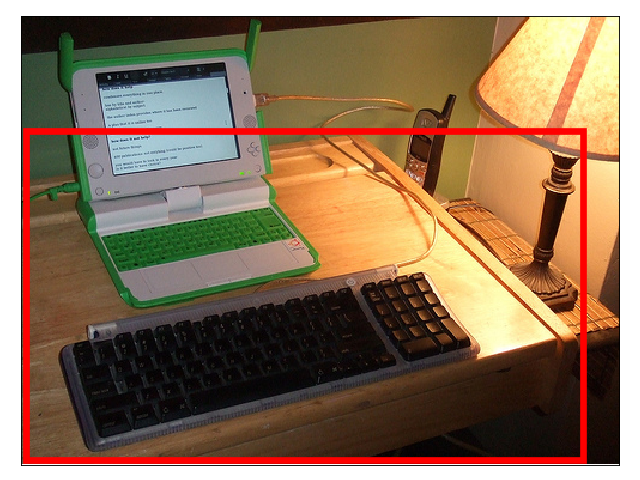
\includegraphics[width=0.9\linewidth]{figures/2320949_1048853_singleton_obj.png}} MN: keyboard  &
%\raisebox{-\totalheight}{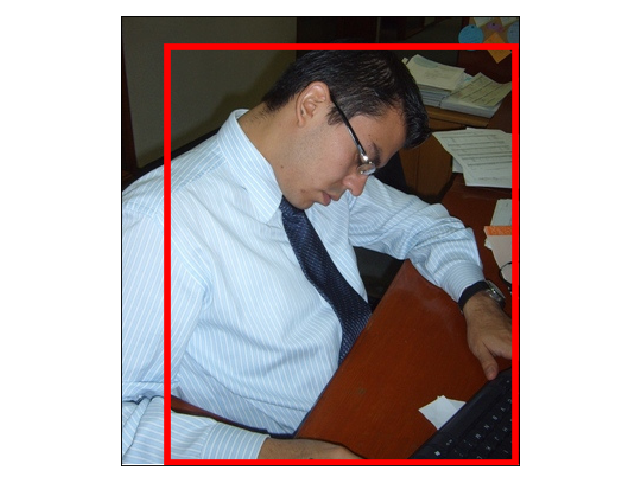
\includegraphics[width=0.9\linewidth]{figures/2343219_926143_supercat_unique.png}}  MN: desktop &
%\raisebox{-\totalheight}{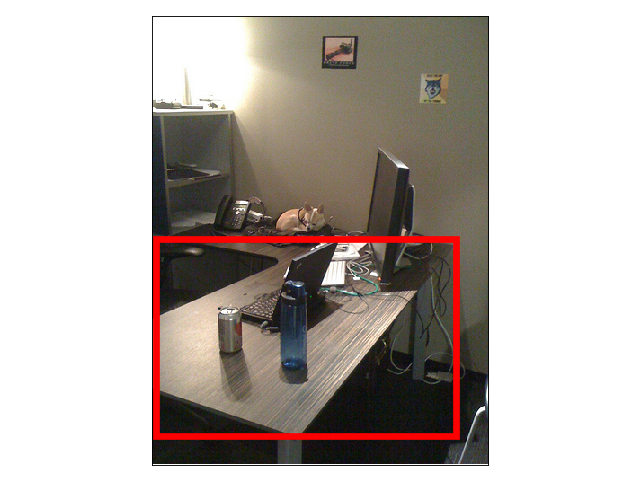
\includegraphics[width=0.9\linewidth]{figures/2354847_1742687_seed_ambiguous.png}} MN: computer \\
%\textbf{bench} &  \raisebox{-\totalheight}{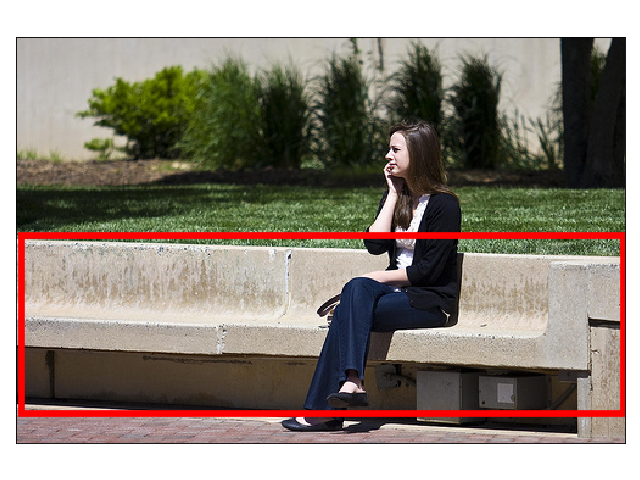
\includegraphics[width=0.9\linewidth]{figures/2350360_1042111_supercat_unique.png}} MN: table  &
%\raisebox{-\totalheight}{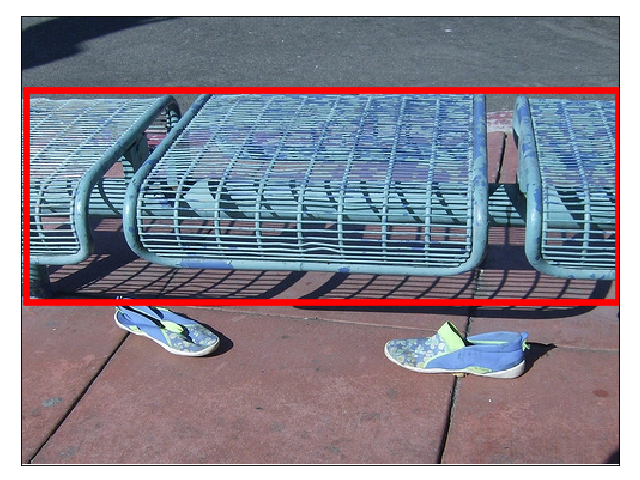
\includegraphics[width=0.9\linewidth]{figures/2389358_1261752_singleton_obj.png}}  MN: seat &
%\raisebox{-\totalheight}{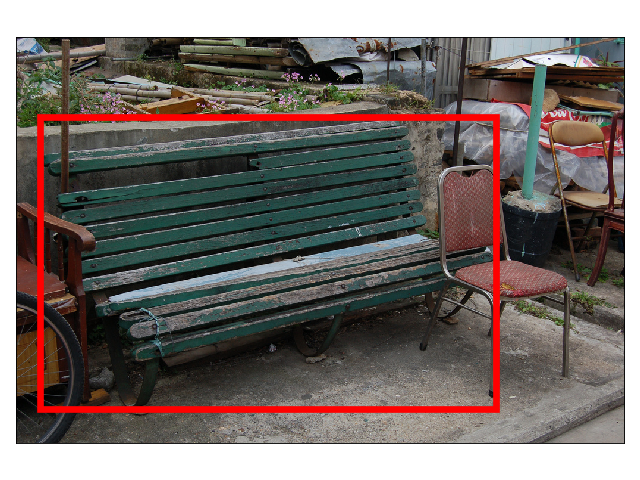
\includegraphics[width=0.9\linewidth]{figures/1593011_2063521_singleton_obj.png}} MN: wood \\
\multicolumn{4}{c}{\textbf{VG: sandwich}}\\
 \raisebox{-\totalheight}{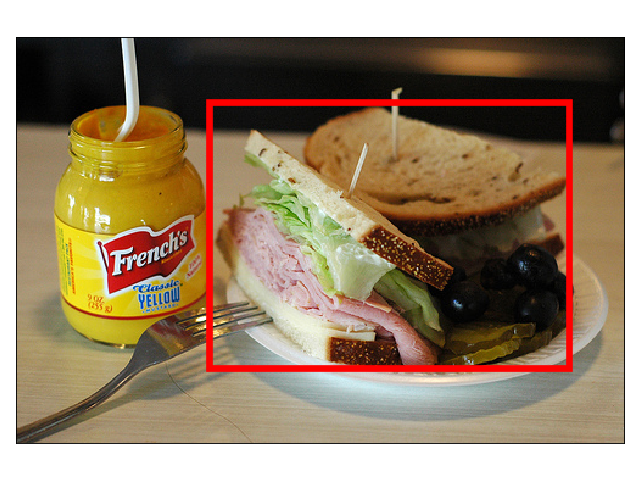
\includegraphics[width=0.9\linewidth]{figures/2339876_3928476_supercat_unique.png}} sandwich (34) &
\raisebox{-\totalheight}{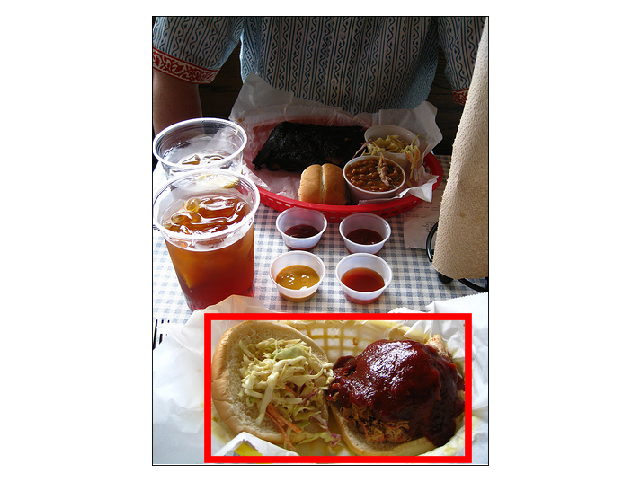
\includegraphics[width=0.9\linewidth]{figures/2379889_1353176_supercat_unique.png}}  sandwich (15), basket (6), food (5), burger (2), hamburger (2), meal (2) &
\raisebox{-\totalheight}{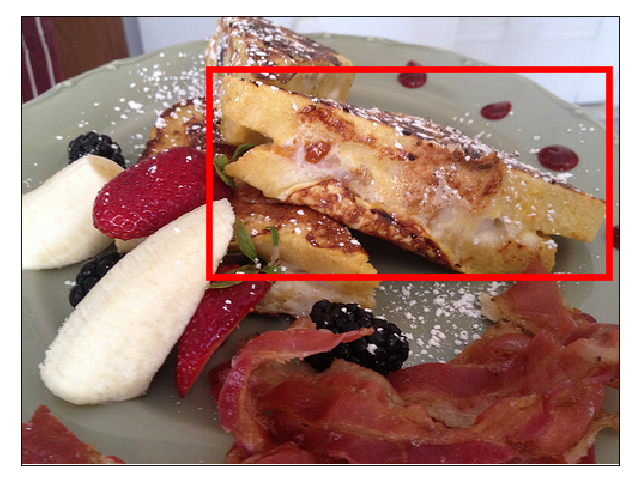
\includegraphics[width=0.9\linewidth]{figures/2394266_465678_singleton_obj.png}} food (10), sandwich (8), toast (5), french toast (4), dessert (2), breakfast (2) &
\raisebox{-\totalheight}{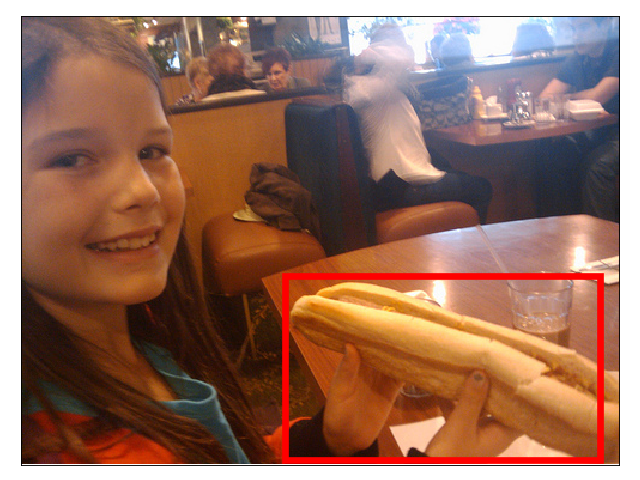
\includegraphics[width=0.9\linewidth]{figures/2386509_681763_supercat_unique.png}} hotdog (14), food (7), bun (4), sandwich (3), bread (2)\\ 
\multicolumn{4}{c}{\textbf{VG: bridge} }\\ 
\raisebox{-\totalheight}{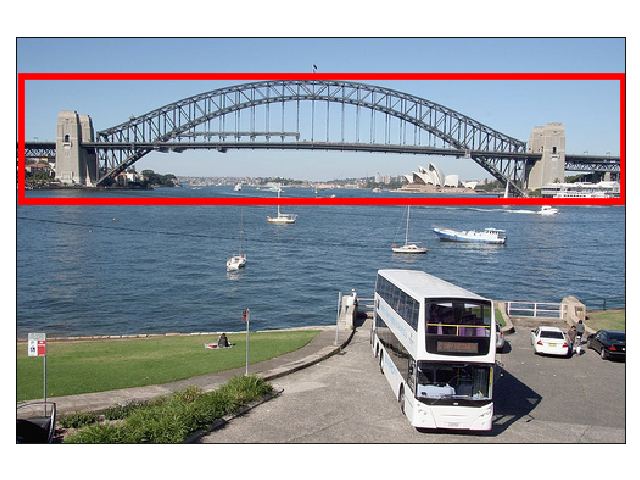
\includegraphics[width=0.9\linewidth]{figures/2341667_2006329_singleton_obj.png}} bridge (35)  &
\raisebox{-\totalheight}{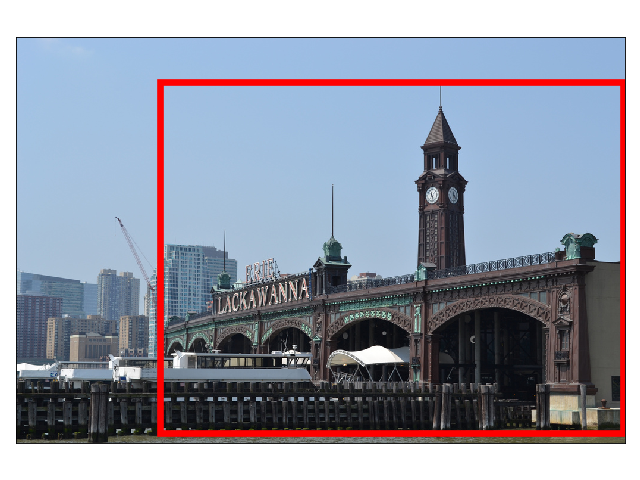
\includegraphics[width=0.9\linewidth]{figures/1592509_1610006_singleton_obj.png}} bridge (20), building (11)  &
\raisebox{-\totalheight}{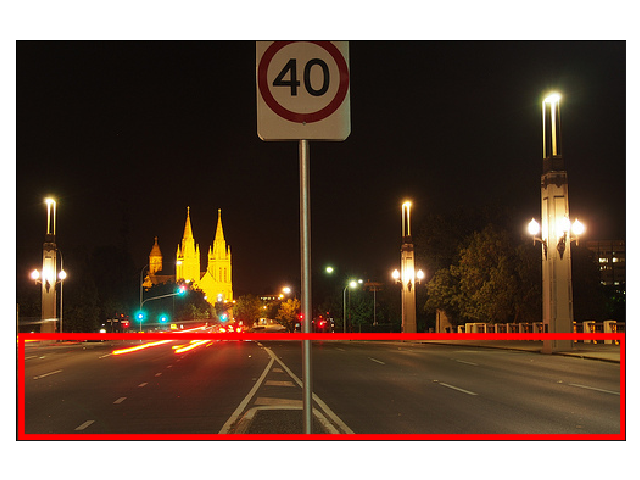
\includegraphics[width=0.9\linewidth]{figures/2384683_1306430_singleton_obj.png}} street (16), road (15), bridge (3) &
\raisebox{-\totalheight}{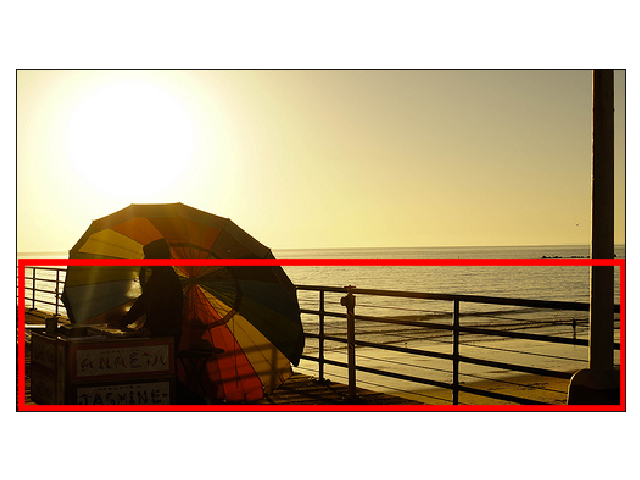
\includegraphics[width=0.9\linewidth]{figures/2412972_3494120_singleton_obj.png}} pier (6), railing (5), dock (5), bridge (5), fence (4), rail (3), boardwalk (3)\\ 
\multicolumn{4}{c}{\textbf{VG: bed}}\\ 
\raisebox{-\totalheight}{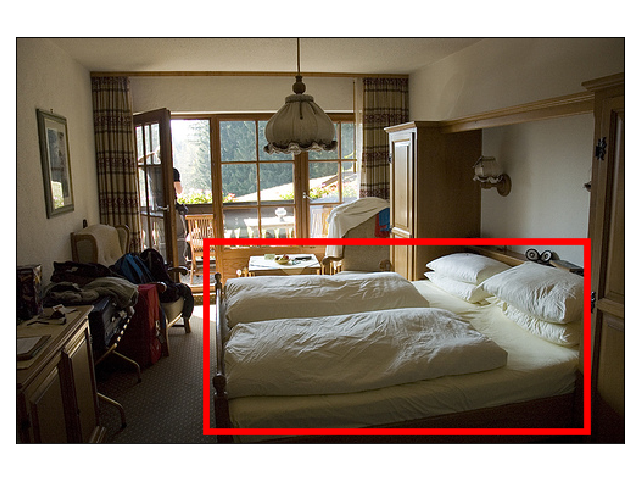
\includegraphics[width=0.9\linewidth]{figures/2321254_3438076_singleton_obj.png}} bed (36)  &
\raisebox{-\totalheight}{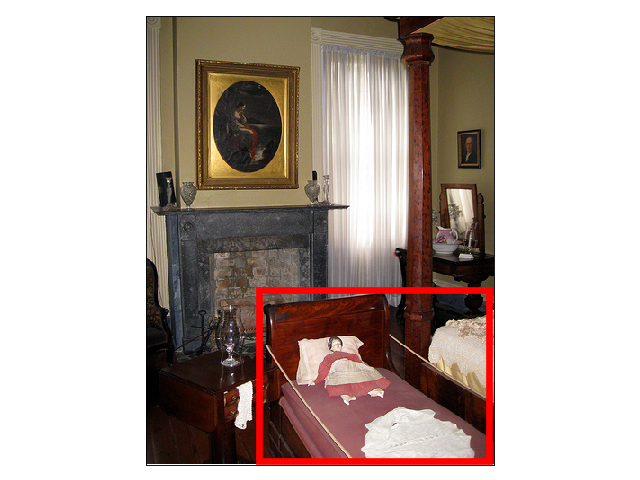
\includegraphics[width=0.9\linewidth]{figures/2324306_3412337_singleton_obj.png}}  bed (16), bench (6), crib (5) &
\raisebox{-\totalheight}{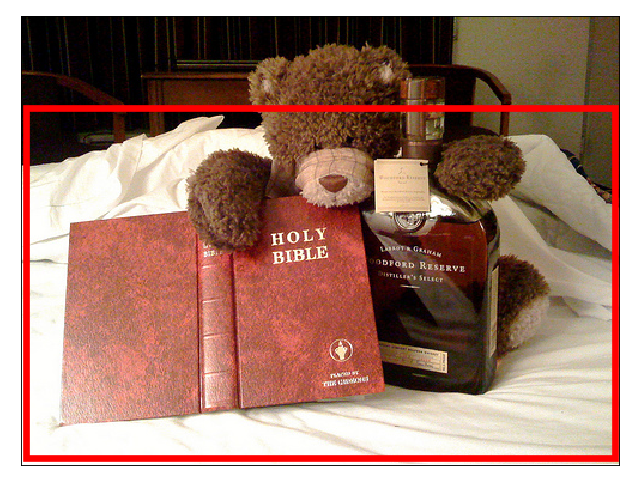
\includegraphics[width=0.9\linewidth]{figures/2342811_3485104_singleton_obj.png}}  bed (17), book (6), table (4), toy (3), bible (2), doll (2) & 
\raisebox{-\totalheight}{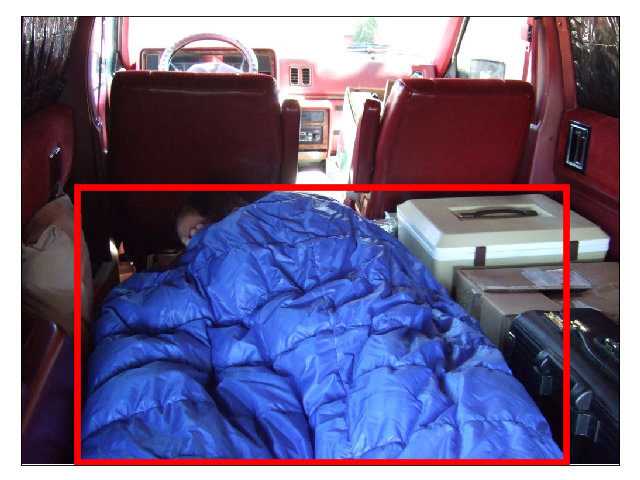
\includegraphics[width=0.9\linewidth]{figures/498222_3135415_singleton_obj.png}} bed (12), sleeping bag (9), blanket (7), bed sheet (5)\\ 
\multicolumn{4}{c}{\textbf{VG: batter}}\\
\raisebox{-\totalheight}{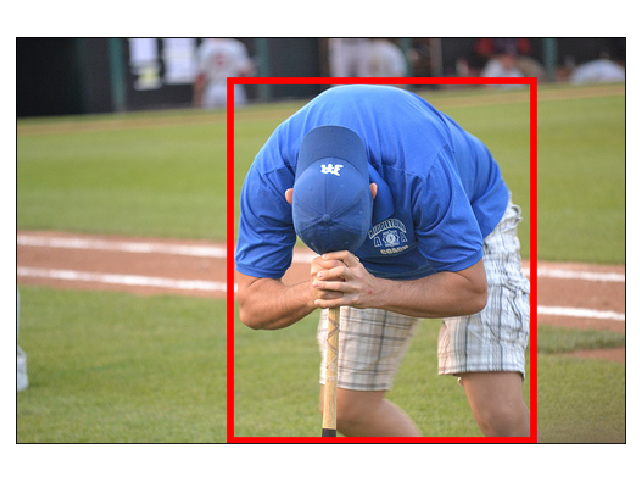
\includegraphics[width=0.9\linewidth]{figures/2372219_2683892_supercat_unique.png}} man (24), cap (5), person (3), baseball player (2) &
  \raisebox{-\totalheight}{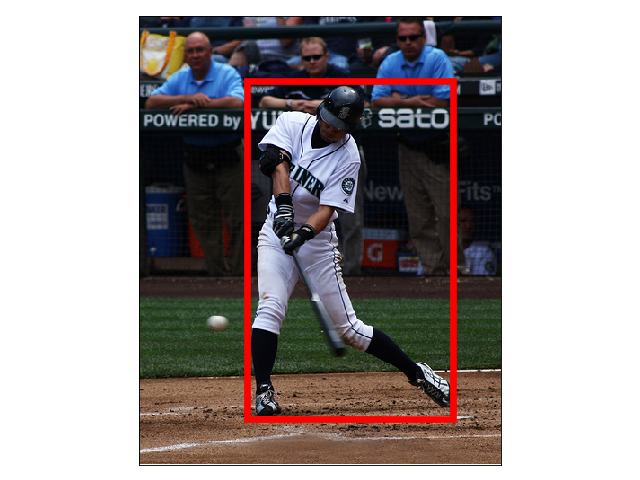
\includegraphics[width=0.9\linewidth]{figures/2394377_464684_singleton_obj.png}} man (13), baseball player (7), batter (5), player (3), helmet (2) &
\raisebox{-\totalheight}{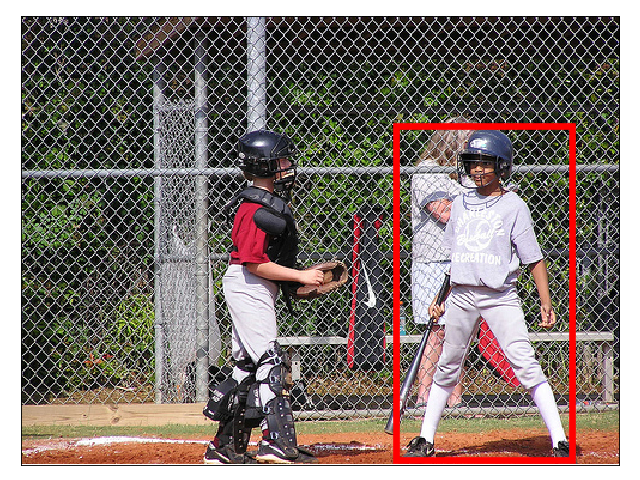
\includegraphics[width=0.9\linewidth]{figures/2398907_2901496_singleton_obj.png}}  boy (7), helmet (5), baseball player (4), player (4), man (3), child (3), batter (3), dress (2), kid (2)&
\raisebox{-\totalheight}{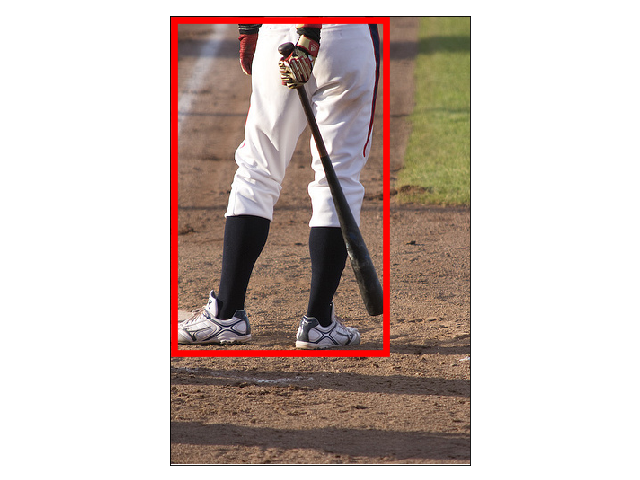
\includegraphics[width=0.9\linewidth]{figures/2337552_957263_singleton_obj.png}} pants (6), player (5), shoe (4), bat (4), person (4), legs (4), baseball player (3), hitter (2)\\ 
\multicolumn{4}{c}{\textbf{VG: robe}}\\
\raisebox{-\totalheight}{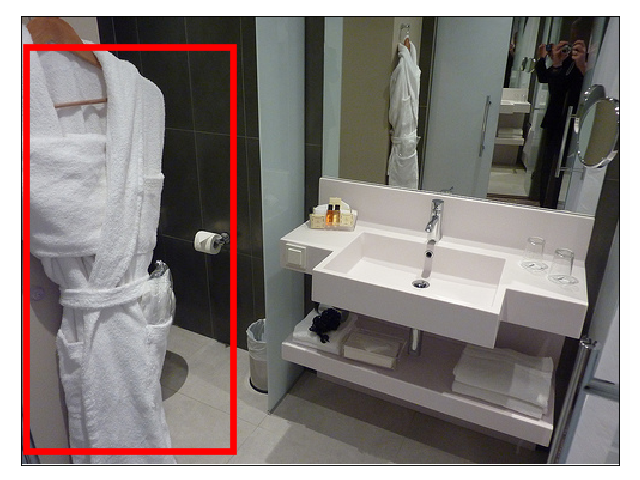
\includegraphics[width=0.9\linewidth]{figures/2373180_2333161_singleton_obj.png}} robe (27), bathrobe (5) &
  \raisebox{-\totalheight}{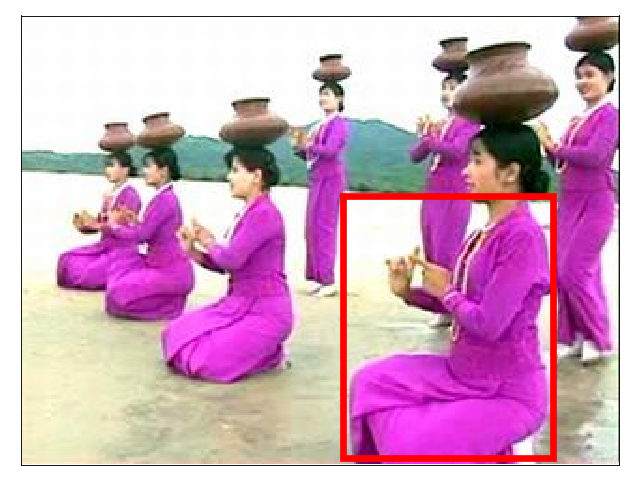
\includegraphics[width=0.9\linewidth]{figures/160_1058761_supercat_unique.png}} dress (30), uniform (2) &
\raisebox{-\totalheight}{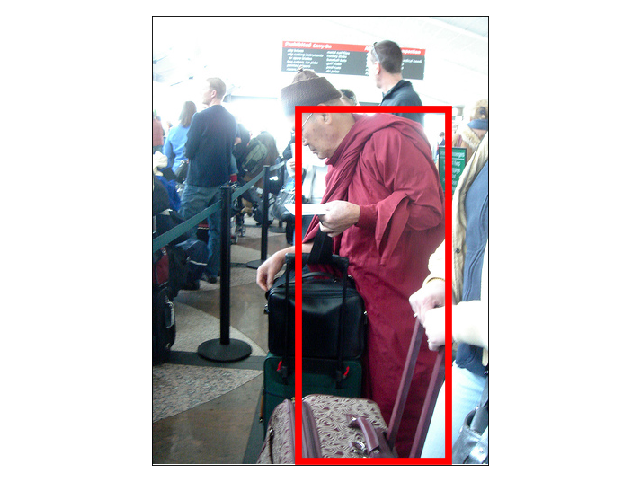
\includegraphics[width=0.9\linewidth]{figures/2334612_2838713_supercat_unique.png}}  robe (11), jacket (7), clothes (6), bag (3), dress (2), man (2) &
\raisebox{-\totalheight}{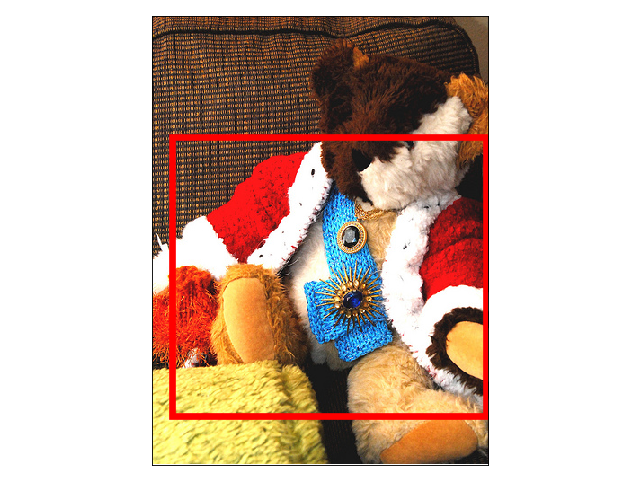
\includegraphics[width=0.9\linewidth]{figures/2340041_2137546_supercat_ambiguous.png}} jacket (10), sweater (9), coat (3), doll (3), toy (3), shirt (2), bear (2), robe (2)\\ 


\end{tabular}

}
\end{minipage}

 \caption{\label{fig:ex}Examples for different instances of VG synsets with low and high agreement in MN data set}
\end{figure*}



%\gbt{The non-canon. VG names suggest that people prefer more general names (``car $>$ sedan'', ``horse $>$ pony'', ``tie $>$ necktie''). Could be due to lexical availability (more general \ra more frequent \ra more available). This could be verified (using frequency). Hypothesis: In cases where top name != VG, the VG name is less general. Could be also a more general hypothesis: see if people prefer more frequent names in general.}
%\cs{@Table~\ref{tab:qual} (just wrt presentation) The most interesting blocks are 2 and 3 (canonical VG with min agr.; non-canonical with max agr.)}


\subsection{Discussion (for now)}
What does this discrepancy between the instance-level and category-level agreement in VisualGenome and ManyNames naming choices mean? 
First of all, it suggests that the same original VisualGenome name can trigger very different variants depending on the visual instance, leading to a drastic increase of variants elicited for categories as compared to instances.
Second, this clearly shows that annotators in VG do not generally annotate the most canonical name \cs{but they don't annotate the name, but the description} and that many names annotated for objects in VG do not correspond to the overall most preferred variant. \sz{think more ...}
\gbt{I don't think we can conclude this second part -- we do have the 70\% top=VG figure that says that VG annotators annotate the most canonical name. What this suggests to me is that instance-level properties are more important than category-level properties, somehow.
  That is, there are systematic properties of instances that make them have a single most salient name.
  However, I expect that this result will be very influenced by referential uncertainty (in single images, it will mostly be clear that it's a man, but in some it may be unclear \ra high instance agreement, low category agrement.}
\cs{I don't think that 70\% is high. E.g., the ResNet has a top-1 error rate of 25\% on ILSVRC 2015.}

\cs{(?!?) With respect to implications for L+V  models on language *interpretation*: much lower agreement on object class-level than on instance-level speaks for using very fine-grained object annotations (as done in ILSVRC). 
	However, that naming variants are often not explained/recoverable by hierarchical relations questions in how far models can understand/interpret reference to objects using more general classes (i.e., names), despite being able to recognise an object's very specific class (e.g., ILSVRC synset). (Relevant?!?)}

\begin{table*}
\footnotesize
%\begin{tabular}{p{1.3cm}cccccc|cccccc}
%\toprule
% & \multicolumn{6}{c|}{Instance-level agreement} & \multicolumn{6}{c}{Class-level agreement}\\ 
%           domain & \% top &    $H$ &    N & N$_{>1}$ & top=VG &  \% VG & \% top &    $H$ &     N & N$_{>1}$ & top=VG &  \% VG \\
%\midrule
%            all &  69.7 (22.2) &  1.3 &  5.7 &   2.9 &  72.8  &  58.7  &   52.6 (21.1) &  2.4 &   62.2 &  29.7 &  32.7 (46.9) &  23.5 (27.0)  \\
% \midrule
%         people &  51.9 (18.1) &  2.1 &  8.6 &   4.3 &         49.8 &         32.3 &     43.1 (14.9) &  2.9 &  104.4 &  53.4 &         24.4 &         13.2  \\
% animals\_plants &  91.3 (12.9) &  0.4 &  2.7 &   1.5 &         93.8 &         88.0 &     67.9 (23.5) &  1.5 &   26.7 &  12.4 &         29.5 &         26.2  \\
%       clothing &  63.9 (17.9) &  1.6 &  6.4 &   3.2 &         70.2 &         52.6 &     49.3 (16.6) &  2.6 &   71.7 &  34.1 &         40.5 &         26.1  \\
%       vehicles &  72.0 (19.5) &  1.1 &  4.7 &   2.4 &         71.1 &         60.2 &    54.4 (17.4) &  2.1 &   70.4 &  33.2 &         21.4 &         21.3  \\
%      buildings &  66.9 (20.5) &  1.5 &  6.9 &   3.0 &         72.6 &         55.5 &      46.7 (18.2) &  3.0 &   68.5 &  31.3 &         32.3 &         22.3  \\
%           home &  66.4 (20.5) &  1.5 &  6.3 &   3.1 &         78.5 &         58.8 &     49.6 (18.7) &  2.8 &  103.2 &  48.8 &         45.9 &         30.1  \\
%           food &  71.3 (21.1) &  1.3 &  5.5 &   2.9 &         62.9 &         52.1 &     47.3 (19.5) &  2.5 &   32.1 &  15.2 &         31.1 &         20.8  \\
%\bottomrule
%\end{tabular}

\begin{tabular}{lccccc|ccccc}
\toprule
 & \multicolumn{5}{c|}{Instance-level agreement} & \multicolumn{5}{c}{Class-level agreement}\\ 
          domain &    N &         \%top (std) &          H (std) & top=VG &   \%VG &     N &         \%top (std) &          H (std) & top=VG &   \%VG \\
\midrule
            all &  2.9 &  75.2 (21.9) &  0.9 (0.7) &   72.8 &  62.8 &  29.7 &  56.4 (21.5) &  2.0 (1.0) &   32.7 &  23.4 \\
       vehicles &  2.4 &  76.6 (19.8) &  0.8 (0.6) &   71.1 &  63.9 &  33.2 &  57.4 (17.3) &  1.8 (0.6) &   21.4 &  21.2 \\
      buildings &  3.0 &  74.7 (20.7) &  1.0 (0.7) &   72.6 &  61.6 &  31.3 &  51.0 (18.8) &  2.4 (0.9) &   32.3 &  22.2 \\
       clothing &  3.2 &  70.1 (18.5) &  1.1 (0.6) &   70.2 &  57.4 &  34.1 &  53.4 (16.6) &  2.1 (0.8) &   40.5 &  26.1 \\
           home &  3.1 &  72.6 (20.7) &  1.0 (0.7) &   78.5 &  64.1 &  48.8 &  54.0 (19.4) &  2.3 (1.0) &   45.9 &  29.9 \\
         people &  4.3 &  59.0 (20.4) &  1.5 (0.7) &   49.8 &  36.3 &  53.4 &  47.5 (17.2) &  2.5 (0.9) &   24.4 &  13.0 \\
           food &  2.9 &  76.4 (20.7) &  0.9 (0.7) &   62.9 &  55.2 &  15.2 &  50.8 (20.3) &  2.0 (0.8) &   31.1 &  20.8 \\
 animals\_plants &  1.5 &  94.5 (12.1) &  0.2 (0.4) &   93.8 &  91.0 &  12.4 &  71.3 (23.3) &  1.2 (0.9) &   29.5 &  26.1 \\
\bottomrule
\end{tabular}

\caption{Agreement in naming measured on the level of instances and on the level of VG classes (i.e.\ after grouping objects by their VG synset), for filtered response sets (frequency threshold of 2)}
\label{tab:agree}
\end{table*}


%Why is naming more flexible in certain domains than in others? \gbt{Hypothesis: expectation: little variation - hypernymy at most, more variation <-> more affordances <-> more varied relationships.}



\cs{@Table~\ref{tab:agree} I still think that we could also have \%\ top with $N>1$ to give an idea as to how useful the data is for the people interested in using it for, e.g., model evaluation. For that, it is clear that crowdsourcing is noisy and before using it some outlier removal needs to be made.}

% \subsection{Entry-level names and preference orders....}

% \sz{an interesting example:} In our data set, there are 24 images where \textit{penguin} has been used, so we know that the object is a \textit{penguin}. For 50\% of these images, annotators still prefer \textit{bird} as the most common name. According to the theory of entry-level categories, this should not happen. People should always prefer \textit{penguin} over \textit{bird}. 

% \sz{how can we analyze this quantitatively?}

% \begin{itemize}
% \item lettuce -- salad
% \item fruit -- food
% \item man -- catcher
% \item bowl --chili
% \item bowl -- diner \gbt{spelling mistake? should be dinner?} 
% \item burger -- meat
% \item statue -- animal (image shows statue of an animal)
% \item bottle -- alcohol
% \item donut --desert \gbt{spelling mistake? should be dessert?} 
% \item zebra -- stripes
% \item oven -- grill
% \end{itemize}


%%% Local Variables:
%%% mode: latex
%%% TeX-master: "main"
%%% End:


\section{Analysis: Taxonomy}
\label{sec:taxo}

\subsection{Lexical relations}

In this section, we take a closer look at the lexical variation we observe in our data set. We analyze the data points where participants attributed different names to the same object and extract a set of  pairwise \textbf{naming variants}. These naming variants correspond to pairs of words that can be used interchangeably to name certain objects.
For each object, we extract the set of naming variants $s = \{ (w_{top},w_2), (w_{top},w_3), (w_{top},w_4),... \}$  where $w_{top}$ is the most frequent name annotated for the object and $w_2 ... w_n$ constitute the less frequent alternatives of $w_{top}$.  The  \textbf{type frequency} of a naming variant $(w_{top},w_x)$ corresponds to the number of objects where this variant occurs. The \textbf{token frequency} of $(w_{top},w_x)$ corresponds the count of all annotations where $w_x$ has been used instead of $w_{top}$.
In Table \ref{tab:exvariants}, we show the the naming variants with the highest raw token frequency for each domain. 

The naming variants can be grouped according to their lexical relation, as follows:

\begin{itemize}
\item \textbf{synonymy}: e.g.\ aircraft vs. airplane 
\item \textbf{hyponymy}: e.g.\ man vs. person
\item \textbf{co-hyponymy}: e.g.\ swan vs. goose
\item \textbf{no relation}: e.g.\  desk vs. apple
\end{itemize}

\begin{table*}

%\begin{tabular}{lll}
%\toprule
%       relation &  types & tokens \\
%\midrule
%synonymy &  0.01 &  0.09 \\
%co-hyponymy &  0.03 &  0.07 \\
%hypernymy &  0.06 &  0.35 \\
%not-covered &  0.19 &  0.04 \\
%crossclassified &  0.70 &  0.47 \\
%\bottomrule
%\end{tabular}
% \small
% \begin{tabular}{llll}
% \toprule
%         relation & \% types & \% tokens & av. depth \\
% \midrule
%  co-hyponymy (closure, max depth=10) &  0.889 &  0.551 &       3.479 \\
%     hyponymy (closure, max depth=10) &  0.097 &  0.328 &       2.204 \\
%         synonymy &  0.015 &  0.121 &       1.000 \\
% \bottomrule
% \end{tabular}

\begin{tabular}{l|ll|ll|ll|ll|ll}
\toprule
      & \multicolumn{2}{c}{crossclassified} & \multicolumn{2}{c}{co-hyponymy} & \multicolumn{2}{c}{hypernymy} & \multicolumn{2}{c}{not-covered} & \multicolumn{2}{c}{synonymy} \\
         domain & typ & tok & typ & tok & typ & tok & typ &  tok & typ & tok \\
\midrule
 people &  0.725 &  0.618 &  0.019 &  0.032 &  0.051 &  0.293 &  0.200 &  0.038 &  0.005 &  0.019 \\
 clothing &  0.709 &  0.661 &  0.020 &  0.046 &  0.045 &  0.195 &  0.219 &  0.085 &  0.008 &  0.012 \\
 animals\_plants &  0.679 &  0.461 &  0.032 &  0.102 &  0.111 &  0.365 &  0.167 &  0.058 &  0.011 &  0.014 \\
 food &  0.590 &  0.433 &  0.031 &  0.033 &  0.104 &  0.432 &  0.267 &  0.089 &  0.009 &  0.013 \\
 vehicles &  0.635 &  0.329 &  0.026 &  0.083 &  0.059 &  0.239 &  0.271 &  0.089 &  0.008 &  0.260 \\
 home &  0.672 &  0.644 &  0.026 &  0.072 &  0.040 &  0.130 &  0.254 &  0.097 &  0.009 &  0.057 \\
 buildings &  0.780 &  0.725 &  0.026 &  0.038 &  0.045 &  0.156 &  0.138 &  0.058 &  0.011 &  0.022 \\
 \hline
 all &  0.731 &  0.574 &  0.033 &  0.057 &  0.076 &  0.256 &  0.147 &  0.050 &  0.013 &  0.064 \\
\bottomrule
\end{tabular}


\caption{Lexical relations between naming variants according to WordNet, for the set of name pairs where both words can be found in WordNet and stand in a \sz{should we produce this table for the different domains?} \gbt{yes, please. Maybe do rows domains, columns lexical relations (synymymy, hyponymy, co-hyponymy, other, not in wordnet), with subcolumns for types and tokens? And do percentages over rows -- for each domain, how many of the variants we find fall into each of the classes. This way we'll be able to see differences across domains.}}
\label{tab:rel}
\end{table*}


Research on object naming following the idea of entry-level categories has, essentially, exclusively looked at names that stand in a hierarchical relation (i.e.\ hyponymy/hypernymy).

We use WordNet to extract lexical relations between the naming variants in our data set.
Unfortunately, this means that we have to exclude a certain portion of the data as either (i) one of the name is not covered in WordNet, (ii) we cannot find a lexical relation between the two names (see below). Also, we had to be relatively permissive with respect to the definition of hyponymy/co-hyponymy. 
For instance, to analyze \textit{giraffe} as a hyponym of \textit{animal} we have to look at the closure of the hyponyms of \textit{animal} with a depth of 8 (in WordNet).
\sz{should we call this co-hyponymy or co-hierarchical relation?}

\sz{include Table that reports counts of the naming variants, coverage in WordNet etc.} \gbt{I think it'd be best to put the out-of-wordnet info in the Lexical relations table -- this way we have everything in one place.}

Table \ref{tab:rel} shows the distribution of lexical relations for those naming variants that we were able to analyze with WordNet.
Both in terms of their types and token frequency, the naming variants that instantiate a (loose) co-hyponymy relation are by far the most frequent.
\sz{discuss in more detail, discuss: to what extent is this an artefact of WordNet?}
This is really interesting: most research on object naming, to date, has focussed on hyponymy/hypernymy, i.e. variation that relates to hierarchical relations between object names.
Our data suggests that co-hierarchical variation is really important too.

\subsection{The ``no relation'' case}

We manually annotated the 100 most frequent name pairs in the ``no relation'' case. Table~\ref{tab:crossclass} shows that, in this category, one third of the pairs do refer to the same object, but the relationship is not captured in WordNet. 
Most of these cases are arguably coverage issues of WordNet, which doesn't capture the co-hyponymy of \textit{horse}-\textit{donkey} or the fact that \textit{vehicle} is hypernym of \textit{train}.\gbt{I find this really weird... also some other cases I annotated. It sounds like I should have listened more carefully to Carina when she suggested going down and up in the wordnet hierarchy (cf.\ the example of food-fruit). :/ Maybe we'd capture quite a bit of them if we did a more sophisticated querying of WordNet. To discuss.}
% between \textit{hat}-\textit{beanie}.
However, a substantial group is constituted by names whose denotations overlap even if they don't belong to the same category. These are typically alternative conceptualizations of objects: as a cat or a toy, as a kind of building or its function (\textit{building}-\textit{home}), or as a portion or a kind of food (\textit{pizza-slice}).

Still, 69\% of the annotated pairs arguably do not denote the same object. Here we find problems HUMANS MAKE SAME ``ERRORS'' AS MACHINES -- REFERENTIAL UNCERTAINTY IN THE ABSENCE OF CONTEXT (discuss as planned with Carina).


Interesting name pairs:

\begin{itemize}
\item storefront - store: strictly speaking it's part-whole, but how can one distinguish between the two? 
\item field - grass: same (reverse); how to distinguish?
\item dog - pet (different conceptualizations; classified as ``hypernym.2'')
\item airplane - flight, plane - flight (classified as ``other'').
\end{itemize}


Most of the cases are co-hyponyms with categories that are easily confused, such as \textit{horse}-\textit{donkey}, \textit{truck}-\textit{jeep}.
In some cases, the visual cues are not enough to distinguish between the categories, but the frequency of this phenomenon suggests that co-hyponyms can be used interchangeably.




%\section{Modeling}
%\label{sec:modeling}

\section{Conclusions}
\label{sec:conc}

\bibliographystyle{acl_natbib}
\bibliography{naming}

%\appendix
%\section{Instructions for AMT Experiment}
%\label{app:instructions}
%
\begin{figure*}
	\centering
	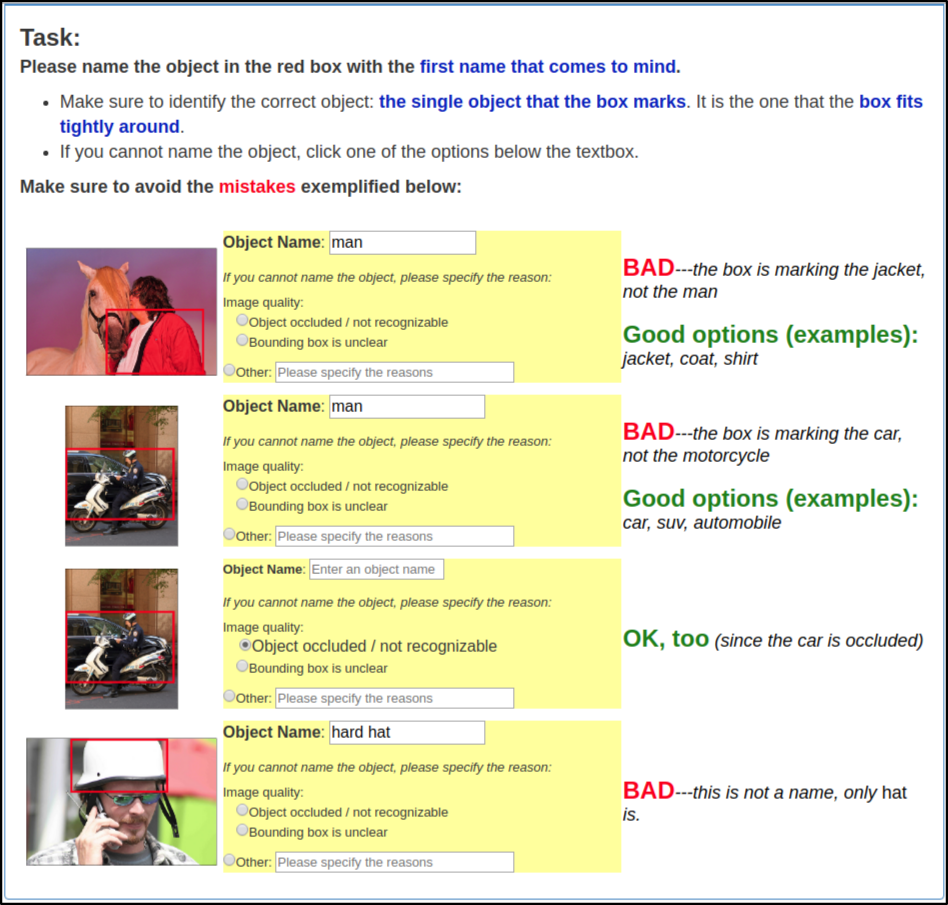
\includegraphics[width=2\columnwidth]{figures/round0.png}
	\caption{Instructions for AMT annotators for round~$0$.}
\end{figure*}

\begin{figure*}
	\centering
	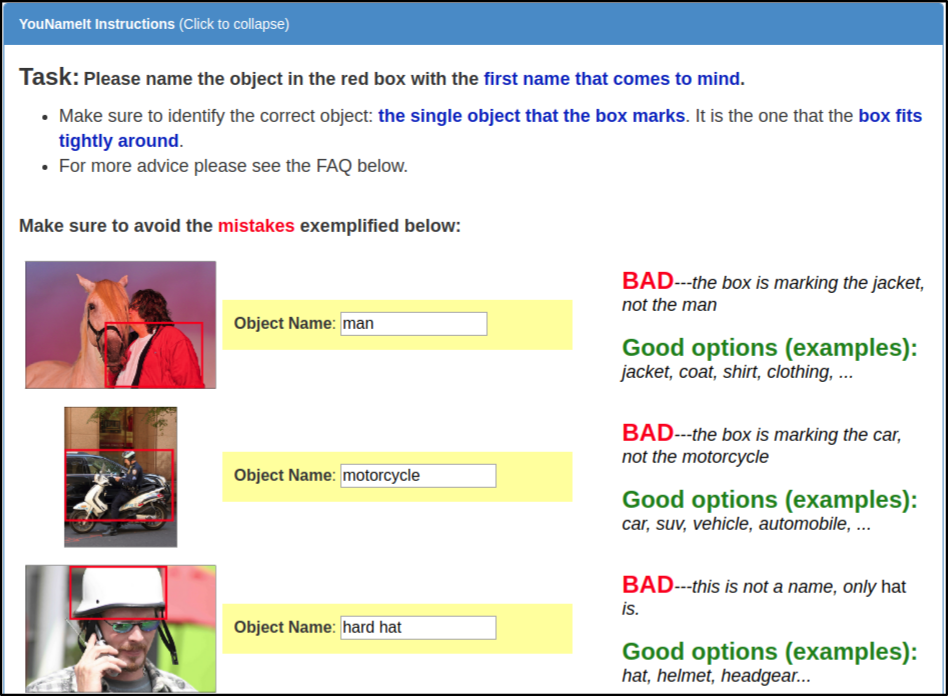
\includegraphics[width=2\columnwidth]{figures/round1+_p1.png}
	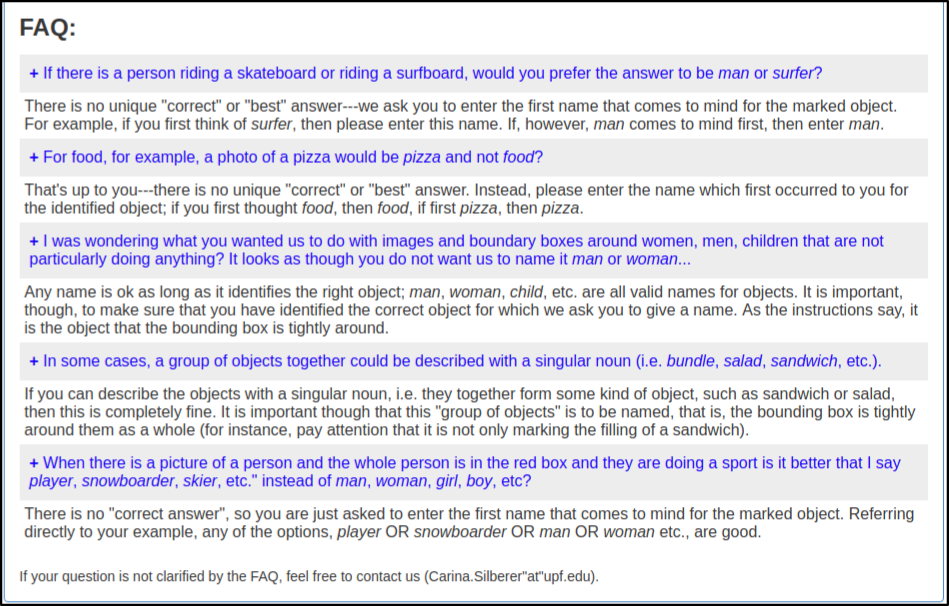
\includegraphics[width=2\columnwidth]{figures/round1+_p2.png}
	\caption{Instructions for AMT annotators for rounds~$1$ to~$3$.}
\end{figure*}

\end{document}


%%% Local Variables:
%%% mode: latex
%%% TeX-master: t
%%% End:
